\documentclass{article}
\usepackage{amsmath,amssymb,graphicx}
\usepackage[margin=1in]{geometry}
\usepackage[colorlinks=true,linkcolor=blue,citecolor=blue,urlcolor=blue]{hyperref}

\newcommand{\dNeff}{\Delta N_{\mathrm{eff}}}
\newcommand{\Tnu}{T_{\nu,\mathrm{dec}}}

\title{A simple CMB $\dNeff$ for the $(\chi,\phi)$ sector}
\author{documentation of \texttt{combined/neff\_simple.m}}
\date{}

\begin{document}
\maketitle

\section{Formula}

A species in equilibrium with the $\gamma+e^\pm$ plasma when neutrinos decouple
(at $\Tnu \simeq 2$~MeV) hands its entropy to the photons, not the neutrinos,
once it goes non-relativistic. This lowers $N_{\rm eff}$ \cite{Boehm:2013jpa}:
\begin{equation}
  N_{\rm eff} \simeq 3.046\left[1 + \frac{7}{22}\sum_i w_i\,\frac{g_i}{2}\,F_i(y_i)\right]^{-4/3},
  \qquad y_i = \frac{m_i}{\Tnu},
\end{equation}
\begin{equation}
  F(y) = \frac{30}{7\pi^4}\int_y^\infty d\xi\,
         \frac{(4\xi^2-y^2)\sqrt{\xi^2-y^2}}{e^\xi \pm 1}
  \qquad (+\ \text{fermion},\ -\ \text{boson}).
\end{equation}
$F$ is the species' entropy in units of one massless Weyl-pair fermion, so
$F_{\rm F}(0)=1$ and $F_{\rm B}(0)=8/7$. We use $g_\phi=1$ and $g_\chi=4$ (Dirac) degrees of freedom; $g_x$ is the $\phi\bar\chi\chi$ coupling and $\mathbf g=(g_u,g_d,g_s)$ the quark couplings,
and quote $\dNeff = N_{\rm eff}-3.046$. Massless limits: $\phi$ alone gives
$X = 2/11$ and $\dNeff=-0.61$; $\chi$ alone gives $X=7/11$ and $\dNeff=-1.47$;
both give $X = 9/11$ and $\dNeff=-1.67$, where $X$ is the bracketed sum.

\section{Which species count}

Each species enters with a weight for its contact with the plasma around $\Tnu$:
equilibrated by $\Tnu$, times still in contact after it,
\begin{equation}
  w_i = \left[1 - e^{-\int_{\Tnu}^{T_{\rm RH}} \frac{\Gamma_i}{H}\frac{dT}{T}}\right]
        \left[1 - e^{-\int_{\Tnu/100}^{\Tnu} \frac{\Gamma_i}{H}\frac{dT}{T}}\right].
\end{equation}
\begin{itemize}
\item $\phi$: inverse decay, $\Gamma_{\rm inv} = \Gamma_{\gamma\gamma}\,K_1/K_2(m_\phi/T)$.
  $\Gamma_{\rm inv}/H$ grows as $T$ falls, so the second factor is $\simeq 1$ and the first
  decides. For light $\phi$, $\Gamma_{\rm inv}/H \propto \eta^2 m_\phi^4$: the threshold sits
  at $m_\phi \propto \eta^{-1/2}$, independent of $g_x$.
  Added to it is the per-$\phi$ rate of $\gamma\gamma\leftrightarrow\phi\phi$. For
  S$\otimes$S/P$\otimes$S this is the charged-meson loop (boxes plus seagull triangle,
  \texttt{notes/gg\_phiphi\_box.tex}), $\sigma=\alpha^2Y^2s\beta/(36864\pi^3)$ with
  $Y=\sum_j\mu_j^2/m_j^4$; for light $\phi$ its rate goes as $\eta^4T^5$, so
  $\Gamma/H\propto\eta^4T^3$ falls with $T$ and it couples $\phi$ from
  $\eta\sim10^{-2}$ for any $m_\phi\ll\Tnu$. Other models use photon exchange,
  $\mathcal O(\alpha)$ smaller (\texttt{notes/gg\_to\_phiphi.tex}).
\item $\chi$: $\Gamma_\chi = \max\!\big(\Gamma_{\gamma\gamma\leftrightarrow\bar\chi\chi},\,
  \min(n_{\chi,\rm eq}\langle\sigma v\rangle_{\bar\chi\chi\to\phi\phi},\,\Gamma_{\rm inv})\big)$,
  i.e.\ directly to photons or through $\phi$. $\Gamma_\chi/H$ falls as $T$ falls, so
  the first factor is $\simeq 1$ and the second decides.
\end{itemize}

\section{$\phi$ made by $\chi$: dark radiation}

$\phi$ not held by the photons can still be made by $\chi$
($\bar\chi\chi\to\phi\phi$, and $\bar\chi\chi\to\phi$ when $m_\phi > 2m_\chi$), then
free-stream as radiation. This runs when $w_\chi^{(1)}(1-w_\phi) > 10^{-10}$, where
$w_\chi^{(1)}$ is the first factor of $w_\chi$ alone: $\chi$ makes $\phi$ even if
it loses contact before $\Tnu$.

\paragraph{Energy equation.} With $\chi$ in equilibrium at $T_\gamma$,
\begin{equation}
  \dot\rho_\phi + 4H\rho_\phi = C_E\left(1 - \frac{\rho_\phi}{\rho_{\phi,\rm eq}}\right),\qquad
  C_E = n_{\chi,\rm eq}^2\langle\sigma v E\rangle_{\bar\chi\chi\to\phi\phi}
      + \Gamma_{\chi\chi}\,m_\phi\,n_{\phi,\rm eq}.
\end{equation}
$C_E$ is the energy $\chi$ puts into an empty $\phi$ population per volume and time:
$\bar\chi\chi\to\phi\phi$, and inverse decay by detailed balance with each $\phi$
carrying $m_\phi$ (boost neglected). The factor $(1-\rho_\phi/\rho_{\phi,\rm eq})$
switches on the reverse processes. It is exact for $\rho_\phi\ll\rho_{\phi,\rm eq}$
(freeze-in) and stops production at equilibrium; in between it interpolates.
Multiplying by $a^4$, with $Q=\rho_\phi a^4$, $a = 1/T_\nu$ and
$dt = d\ln(1/T_\gamma)/H$,
\begin{equation}
  \frac{dQ}{d\ln(1/T_\gamma)} = k\,(Q_{\rm eq} - Q),\qquad
  k = \min\!\left(\frac{C_E}{H\rho_{\phi,\rm eq}},\ \frac{\Gamma_\chi}{H}\right).
\end{equation}
The $\min$ is the chain bottleneck: energy reaches $\phi$ from the photons through
$\chi$, so no faster than $\chi$'s own photon link $\Gamma_\chi$ (Sec.~2). The
target is $Q_{\rm eq} = (1-w_\phi)\,\rho_{\phi,\rm eq}(T_\gamma)\,a^4$: the fraction
$w_\phi$ is already in $X$ through the photon link. The equation runs from
$T_{\rm RH}$ to $\min(\Tnu/100,\,m_\chi/50)$; below that $n_{\chi,\rm eq}$ is
negligible, $k\to0$ and $Q$ is frozen.

\paragraph{Entropy balance.} Eq.~(1) sends all the entropy of the contact species to
the photons; the part $\phi$ takes away is not. After $\Tnu$ the neutrinos are
decoupled, and the entropy of the photon bath plus $\phi$ is conserved; making $\phi$
from $\chi$ moves entropy from one to the other. In units of $T_\nu^3$, with photons
counting 2,
\begin{equation}
  g_{\star s}^{\rm bath}(T_\gamma)\left(\frac{T_\gamma}{T_\nu}\right)^3 + s_\phi(Q) = S_i,
  \qquad S_i = \frac{11}{2}(1+X) + s_\phi(Q)\big|_{\Tnu},
\end{equation}
\begin{equation}
  g_{\star s}^{\rm bath}(T) = 2 + \tfrac72 F_{\rm F}\!\left(\tfrac{m_e}{T}\right)
    + w_\chi\,\tfrac78 g_\chi F_{\rm F}\!\left(\tfrac{m_\chi}{T}\right)
    + w_\phi\,\tfrac78 g_\phi F_{\rm B}\!\left(\tfrac{m_\phi}{T}\right),
  \qquad s_\phi = g_\phi\left(\frac{30\,Q}{\pi^2 g_\phi}\right)^{3/4}.
\end{equation}
$S_i - s_\phi|_{\Tnu} = g_{\star s}^{\rm bath}(\Tnu)$: $\gamma+e^\pm$ give $11/2$ and
$(11/2)X = \tfrac78\sum_i w_i g_i F_i$ the contact species. $s_\phi = g_\phi
(T_\phi/T_\nu)^3$ for a thermal-shape $\phi$ with $Q = \tfrac{\pi^2}{30} g_\phi
(T_\phi/T_\nu)^4$. The balance gives $T_\gamma/T_\nu$ at each step, which sets
$a = 1/T_\nu$ in $Q_{\rm eq}$, so $Q$ and $T_\gamma/T_\nu$ are stepped together.

\paragraph{Decay before recombination.} $\phi$ that decays to SM states
($\gamma\gamma$, and $\pi\pi$, $K\bar K$ where open) before recombination returns
its entropy to the photons. Its surviving fraction is
\begin{equation}
  P = \exp\!\left[-\int_{T_{\rm rec}}^{\Tnu} \frac{\Gamma_{\rm SM}}{H}\,
      \frac{K_1}{K_2}\!\left(\frac{m_\phi}{T_\gamma}\right)\frac{dT_\gamma}{T_\gamma}\right],
\end{equation}
with $\Gamma_{\rm SM}=\Gamma_{\gamma\gamma}+\Gamma_{\rm meson}$ and the time dilation taken at $T_\gamma$. $Q_f = P\,Q$ replaces $Q$ in the final
balance, so the decayed fraction's entropy lands in the bath:
$(T_\gamma/T_\nu)^3_{\rm rec} = [S_i - s_\phi(Q_f)]/2$.

\paragraph{$N_{\rm eff}$.}
\begin{equation}
  N_{\rm eff} = 3.046\left[\tfrac{4}{11}\left(\tfrac{T_\gamma}{T_\nu}\right)^3\right]^{-4/3}
  + \frac{R(y)\,\rho_\phi}{\rho_{1\nu}},
\end{equation}
where $\rho_{1\nu} = \tfrac78\tfrac{\pi^2}{15}\big[(4/11)^{1/3}T_\gamma\big]^4$ is one
Standard-Model neutrino at the same $T_\gamma$, the reference that defines
$N_{\rm eff}$. $R(y) = \int (E-m_\phi)\,p^2 f\,dp \big/ \int p^3 f\,dp$ is the
kinetic fraction of a $\phi$ that decoupled relativistically ($f$ Bose--Einstein in
$p/T_\phi$), at $y = m_\phi/T_\phi$ at recombination, with
$T_\phi = (30Q_f/\pi^2 g_\phi)^{1/4}\,T_\nu$. $Q = 0$ gives back Eq.~(1).

\paragraph{Check.} Massless $\phi$ with no photon link ($w_\phi=0$), thermalised
through a light $\chi$ ($w_\chi = 1$) that outlives $e^\pm$ annihilation. At $\Tnu$,
$T_\phi = T_\gamma = T_\nu$, so $s_\phi = 1$ and
$S_i = \tfrac{11}{2} + \tfrac78\cdot4 + 1 = 10$. After $e^\pm$ and $\chi$ annihilate
with $\phi$ tracking $T_\gamma$: $(2+1)(T_\gamma/T_\nu)^3 = 10$, so
$T_\phi = T_\gamma = (10/3)^{1/3}T_\nu$. Then
$N_{\rm eff} = 3.046\,(40/33)^{-4/3} + \tfrac47(11/4)^{4/3} = 2.357 + 2.201$, and
$\dNeff = +1.51$.

\paragraph{Caveats.}
(i) $\chi$ and the $\phi$ it makes are taken at $T_\gamma$; a dark bath at its own
temperature is only approximated through the bottleneck.
(ii) $s_\phi$ assumes a thermal-shape $\phi$.
(iii) Partial contact is taken to mean partial entropy transfer.
(iv) The relaxation form interpolates between freeze-in and equilibrium.
(v) Each inverse-decay $\phi$ carries $m_\phi$.

\section{Results}

All figures use \texttt{heavyScalar} and $\mathbf g = \eta\,[1,1,1]/3$. The shaded
band is the Planck $2\sigma$ range, $\dNeff = -0.054 \pm 0.34$.

\begin{figure}[h]
  \centering
  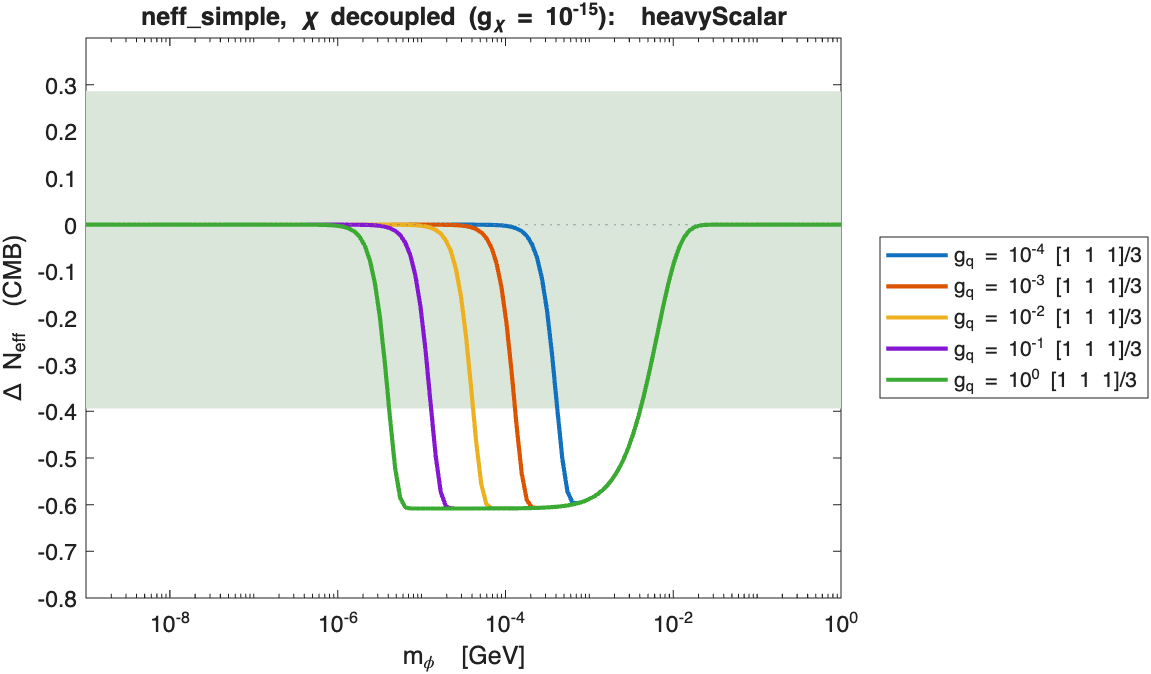
\includegraphics[width=0.8\textwidth]{neff_simple_figs/neff_simple_vs_mphi_gq.png}
  \caption{$\phi$ only ($g_x = 10^{-15}$), $m_\chi = 1$~MeV. The lower edge
  moves as $\eta^{-1/2}$. The upper edge, $m_\phi \sim \Tnu$, is where $\phi$ carries
  no entropy, whatever $\eta$.}
\end{figure}

\begin{figure}[h]
  \centering
  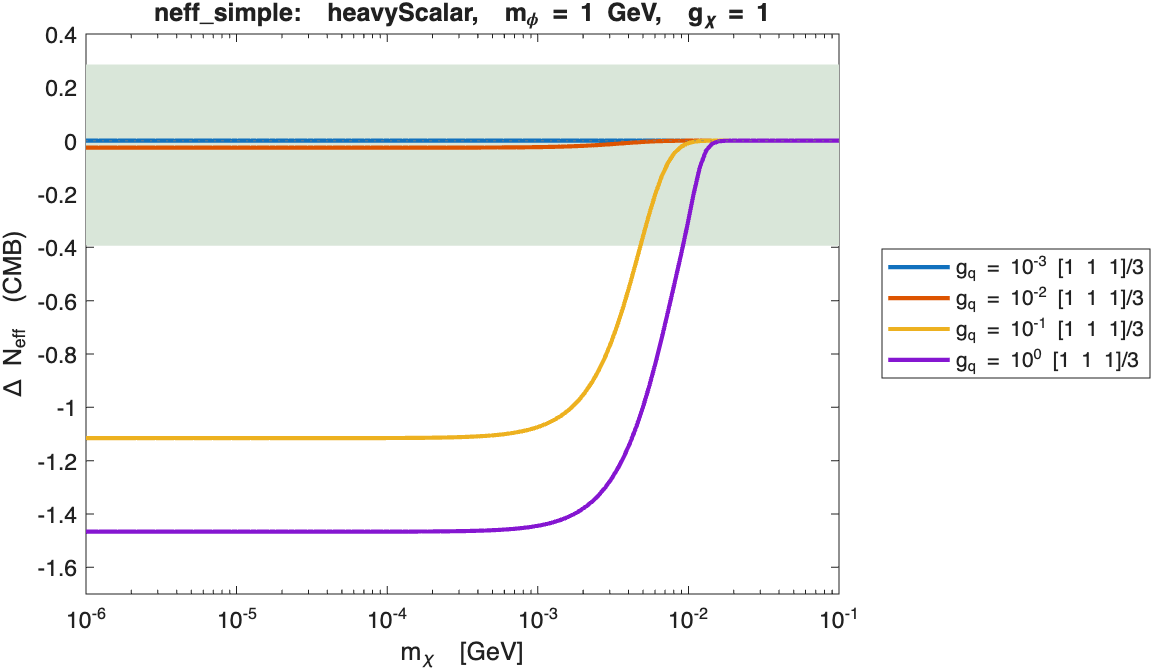
\includegraphics[width=0.8\textwidth]{neff_simple_figs/neff_simple_vs_mx.png}
  \caption{Heavy $\phi$ ($m_\phi = 1$~GeV, $g_x = 1$): only $\chi$ contributes.
  For $\eta \le 10^{-2}$, $\chi$ is barely in contact; for $\eta = 0.1$ it is partly
  in contact ($-1.12$ rather than $-1.47$). The rise above $m_\chi \sim 1$~MeV is
  $F_{\rm F}(m_\chi/\Tnu)\to 0$.}
\end{figure}

\begin{figure}[h]
  \centering
  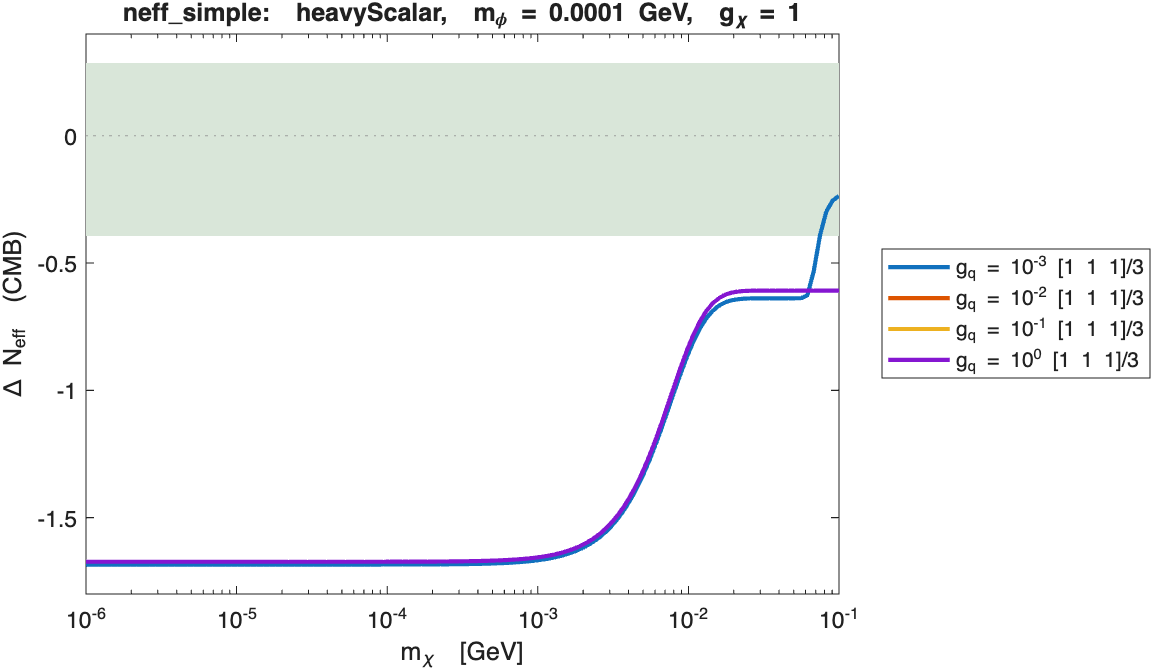
\includegraphics[width=0.8\textwidth]{neff_simple_figs/neff_simple_vs_mx_lightphi.png}
  \caption{Light $\phi$ ($m_\phi = 0.1$~MeV, $g_x = 1$). For light $\chi$ the
  curves coincide at $-1.67$, falling to $\phi$'s $-0.61$. For $\eta = 10^{-3}$ the
  photon link gives $w_\phi = 0.28$; $\chi$ supplies the rest of $\phi$ unless it is
  too heavy ($m_\chi \gtrsim 60$~MeV).}
\end{figure}

\begin{figure}[h]
  \centering
  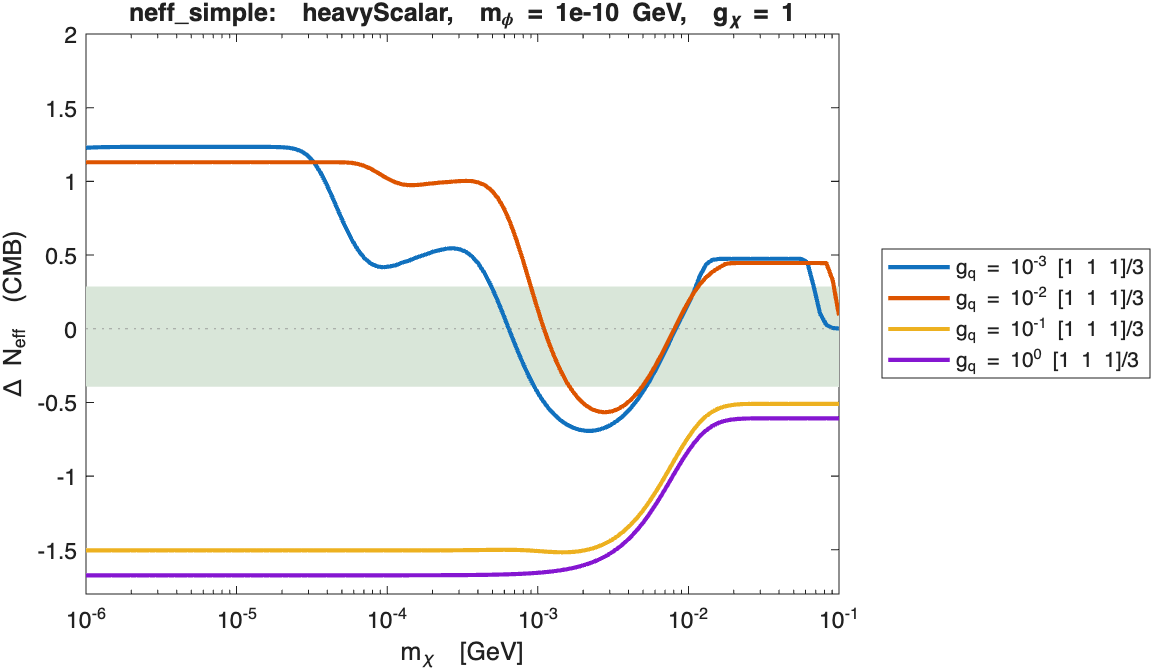
\includegraphics[width=0.8\textwidth]{neff_simple_figs/neff_simple_vs_mx_ultralightphi.png}
  \caption{Ultralight $\phi$ ($m_\phi = 10^{-10}$~GeV, $g_x = 1$). For
  $\eta \le 10^{-2}$, $\phi$ made by $\chi$ survives as radiation: $\dNeff > 0$,
  $+0.47$ once $\phi$ decouples before $e^\pm$ annihilation ($+0.57$ reduced by
  $\phi$ being partly non-relativistic at recombination). For $\eta \ge 0.1$, $\phi$
  decays to photons before recombination and its entropy heats them.}
\end{figure}

\begin{thebibliography}{9}
\bibitem{Boehm:2013jpa}
C.~Boehm, M.~J.~Dolan and C.~McCabe,
``A lower bound on the mass of cold thermal dark matter from Planck,''
JCAP \textbf{08} (2013) 041, arXiv:1303.6270.
\end{thebibliography}

\end{document}
